
% This LaTeX was auto-generated from MATLAB code.
% To make changes, update the MATLAB code and republish this document.

\documentclass[11pt]{article}
\usepackage[utf8]{inputenc}
\usepackage[T1]{fontenc}
\usepackage{amsthm}
\usepackage{enumitem}
\usepackage{amssymb}
\usepackage{amsmath}
\usepackage{amsfonts}
\usepackage[version=4]{mhchem}
\usepackage{stmaryrd}
\usepackage{mathrsfs}
\usepackage{bm}
\usepackage{graphicx}
\usepackage[export]{adjustbox}
\graphicspath{ {./images/} }
\usepackage{algorithm}
\usepackage{algorithmic}
\usepackage{makecell}  % 表格换行
\usepackage{tikz}
\usepackage{enumitem}





 \usepackage{hyperref}
\hypersetup{
    colorlinks=true,     % 启用颜色链接
    linkcolor=blue,     % 内部链接的颜色
    citecolor=red,      % 引用文献的颜色
    urlcolor=blue,       % URL链接的颜色
    linktoc=red,      % 不影响目录链接颜色
}
\usepackage[a4paper, top=1in, bottom=1in, left=1in, right=1in]{geometry}

\title{
{\bf \huge FEM: Basic Theory and Implementation}\\
{\bf \large 1-D  FEM for Elliptic Equation}
}
\author{Huaijin Wang}
\date{\today}


\begin{document}


\newtheorem{definition}{Definition}[section]
\newtheorem{property}{Property}[section]
\newtheorem{lemma}{Lemma}[section]
\newtheorem{theorem}{Theorem}[section]
\newtheorem{corollary}{Corollary}[section]
\newtheorem{remark}{Remark}[section]
\newtheorem{example}{Example}[section]
\numberwithin{equation}{section}


\maketitle

\begingroup
\hypersetup{
    linkcolor=black,  % 将目录链接颜色设置为黑色
}
\tableofcontents
\endgroup


\newpage

\section{Introduction}
This notes present Finite Element Method (FEM) for 1d elliptic problem, and aim at the main procedures of such method easily.

\noindent $\bullet$ Why Elliptic problem?

\noindent $\bullet$ Why 1D case?

\noindent $\bullet$ Why FEM?

\section{General Finite Element and Finite Element Spaces}

\subsection{Finite Element}
In the next, we introduce a concept of finite element generally:
\begin{definition}
A triple $(K,\mathcal{P},\mathcal{N})$ is called a \textbf{finite element} if it satisfies the following properties:
\begin{enumerate}[label={\rm (\roman*)}]
\item $K \subset \mathbb{R}^d$ ($d=1,2,3$) is a closed set with piecewise smooth boundary (called the \textbf{element});
\item $\mathcal{P}$ is a finite-dimensional space of functions on $K$ (called the \textbf{space functions});
\item $\mathcal{N}$ is finite set of linear functionals $\mathcal{P}\to \mathbb{R}$ and forms a basis for $\mathcal{P}^\prime$ (called the \textbf{degree of freedom}).
\end{enumerate}
\end{definition}

\begin{remark}
The name finite element is clear due to the finite dimensional space $\mathcal{P}$, which uniquely determined by the DOFs, over an element ${K}$.
\end{remark}





\begin{lemma}
Suppose that $\mathcal{P}$ is finite dimensional and let $\{\psi_1,\cdots,\psi_n\}$ be a basis of $\mathcal{P}$. Then there exists uniquely a set of functionals $\{f_1,\cdots,f_n\}\subset \mathcal{P}^\prime$ such that
\[
f_i(\psi_j) = \delta_{i,j},\quad i,j=1,\cdots,n.
\]
Moreover, $\{f_i\}$ form a basis for $\mathcal{P}^\prime$, which is called the dual basis of $\{\psi_i\}$. Thus $\mathrm{dim} \mathcal{P} = \mathrm{dim} \mathcal{P}^\prime$.
\end{lemma}
\begin{proof}
The coordinate functionals $g_1,\cdots,g_n$ are given by
\[
\left \langle g_i, \sum_{k=0}^n \lambda_k \psi_k \right \rangle = \lambda_i.
\]
Clearly, $g_i\in \mathcal{P}^\prime$. Thus $\langle g_i,\psi_k \rangle = \delta_{i,k}$. Then for any $v\in\mathcal{P}$ we have $\langle g_i-f_i, v\rangle = 0$, which implies $g_i=f_i$.

We now show that $\{f_i\}$ are linearly independent. Indeed, suppose that there exists $a_i\in \mathbb{R}$ such that $\sum_{i=1}^n a_i f_i = 0$, where $0$ denotes the zero functional. Thus
\[
a_k = \sum_{i=1}^n a_i \langle f_i, \psi_k \rangle = \langle 0, \psi_k\rangle = 0,\quad k=1,\cdots,n.
\]
We now show that $\mathcal{P}^\prime = \mathrm{span}\{f_1,\cdots,f_n\}$. For any $f\in \mathcal{P}^\prime$, let $b_i = f(\psi_i)$ for $i=1,\cdots,n$. Thus we have $f = \sum_{i=1}^n b_i f_i$. In fact, by definition 
\[
f(\psi_k) = \sum_{i=1}^n b_i f_i(\psi_k),\quad k=1,\cdots,n,
\]
which implies $f(v) = \sum_{i=1}^n b_i f_i(v),\ \forall v\in \mathcal{P}$.
\end{proof}



\begin{remark}
It is clear that the number of elements in $\mathcal{N}$ is equal to the dimension of $\mathcal{P}$. 
\end{remark}

\begin{remark}
Any function $v \in \mathcal{P}$ is uniquely determined by an arbitrary assignment of values to the DOFs. In fact, suppose that $\mathcal{P} = \mathrm{span}\{\psi_1,\cdots,\psi_n\}$ and $\mathcal{N} = \{\mathcal{N}_1,\cdots,\mathcal{N}_n\}$. Let the dual basis $\mathcal{P}^\prime = \mathrm{span} \{f_1,\cdots,f_n\}$. Then it is clear that $v = \sum_{i=1}^n f_i(v)\psi_i$. We suppose that $\mathcal{N}_i = \sum_{j=1}^n c_{ij} f_j$. Thus
\[
\mathcal{N}_i(v) = \sum_{j=1}^n c_{ij} f_i(v), \ i=1,\cdots,n.
\]
It is known that the matrix $(c_{ij})$ is nonsingular, then the coefficients $\{f_i(v)\}$ of $v$ is uniquely determined by the assignment of values to $\{\mathcal{N}_i(v)\}$. 
\end{remark}

\begin{definition}
Let $(K,\mathcal{P},\mathcal{N})$ be a finite element. A basis $\{\psi_1,\cdots,\psi_n\}$ for $\mathcal{P}$ is called the \textbf{nodal basis} for $\mathcal{P}$ if it is dual to $\mathcal{N}$, i.e., $\mathcal{N}_i (\psi_j) = \delta_{i,j}$.
\end{definition}

\begin{example}
Let $K = (0,1)$, $\mathcal{P}$ be the space of linear polynomials, and $\mathcal{N} = \{ \ell_0, \ell_1 \}$ satisfying
\[
\ell_0 (p) = p(0), \ \ell_1 (p) = p(1),\quad \forall p\in \mathcal{P}.
\]  
The triple $(K,\mathcal{P},\mathcal{N})$ is a finite element. The nodal basis of $\mathcal{P}$ is 
\[
\varphi_0 (x) = 1-x,\quad \varphi_1(x) = x.
\]
\end{example}

\begin{remark}
Why nodal basis?
\end{remark}

The discussion above states a general framework to define a finite element. However, in implementations and many applications, the finite element will be specified as 
\begin{enumerate}[label=(\roman*)]
\item Element $K$ is an interval in $1$d case, a triangle or parallelogram in $2$d case, and a tetrahedron or parallelepiped in $3$d case.
\item $\mathcal{P}$ is a finite dimensional space containing polynomials.
\item $\mathcal{N}$ contains functionals that map $v\in\mathcal{P}$ to $v(p)$ for some $p\in K$ (referred to \textbf{Lagrange} type), or to $D^\alpha v(p)$ for some $p\in K$ and derivatives $D^\alpha$ (referred to \textbf{Hermite} type).
\end{enumerate}

\begin{remark}
\textcolor{blue}{We only consider the Lagrange element, i.e., $\mathcal{P}$ is space of polynomials and $\mathcal{N}$ is Lagrange type.}
\end{remark}

\textcolor{red}{Global Degree of Freedom?}

\subsection{Assembled Finite Element Space}

Let $\{x_n\}_{n=0}^{N+1}$ be a grid on the interval $I=(a,b)$. Each \textbf{element} $I_n=(x_{n-1}, x_{n})$ is the subinterval of $I$ with length of $h_n = |x_{n}- x_{n-1}|$. We also denote $h = \max_{1\leqslant n \leqslant N+1} h_n$, which is a parameter to measure how fine the partition is.


\begin{center}
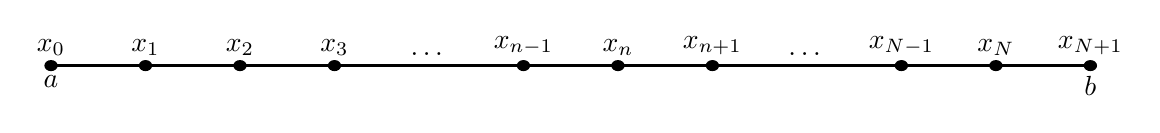
\begin{tikzpicture}[xscale=1.2, yscale=1, thick]
\draw[-] (0,0) -- (11,0);
 \foreach \x in {0,...,3} {
 \fill (\x,0) circle (2pt); % 圆点
 \node[above] at (\x,0) {$x_{\x}$};
 }
 \node[above] at (4,0) {$\dots$};
 \fill (5,0) circle (2pt);
 \node[above] at (5,0) {$x_{n-1}$};
 \fill (6,0) circle (2pt);
 \node[above] at (6,0) {$x_{n}$};
 \fill (7,0) circle (2pt);
 \node[above] at (7,0) {$x_{n+1}$};
 
 \node[above] at (8,0) {$\dots$};
 \fill (9,0) circle (2pt);
 \node[above] at (9,0) {$x_{N-1}$};
 \fill (10,0) circle (2pt);
 \node[above] at (10,0) {$x_{N}$};
 \fill (11,0) circle (2pt);
 \node[above] at (11,0) {$x_{N+1}$};
 
 \node[below] at (0,0) {$a$};
 \node[below] at (11,0) {$b$};
\end{tikzpicture}
\end{center}

Let $\mathcal{T}_h = \{I_n: 1\leqslant n \leqslant N+1\}$, which is called a partition of the interval $I$. The idea to construct the approximation space is by defining a finite element triple $(I_n, \mathcal{P}(I_n), \mathcal{N}(I_n))$ on each element $I_n$, and then assemble them in a way of single-valued DOFs to an \textbf{Assembled Finite Element Space} with the properties: for any $v(x)$ defined on $I$,
\begin{enumerate}[label=(\roman*)]
\item $v|_{I_n} \in \mathcal{P}(I_n)$, $n=1,\cdots,N+1$.
\item If $T_1, T_2\subset \mathcal{T}_h$ and share the same node $p\in \bar{T}_1\cap \bar{T}_2$ that corresponding DOFs applied on, then the corresponding DOFs applied on $v|_{T_1}$ and $v|_{T_2}$ over $p$ are the same value.
\end{enumerate}

The assembled finite element space is denoted as $(\mathcal{T}_h, \mathcal{P}, \mathcal{N})$

\begin{remark}
Theoretically, each $\mathcal{P}(I_n)$ or $\mathcal{N}(I_n)$ may be different. However, this configuration is not suitable for analysis and implementations. We will assume that $\mathcal{P}(I_n) \in \mathbb{P}_k$ for some $k\in \mathbb{N}$. 
\end{remark}

\subsection{$X_h^k$ Space}

\begin{remark}
Compared to $2$ or $3$d cases, the $1$d case is easy to give a partition over $I$.
\end{remark}

We consider the finite-dimensional subspace of $H^1(I)$.


Let $X_h^k$ be the space of piecewise polynomials in $I$, i.e.,
\[
X_h^k := \{v(x) \in C^0(\bar{I}): v  |_{I_n} \in \mathbb{P}_k,\ n=1,\cdots,N+1 \}.
\]


\begin{lemma}
We have $X_h^k \subset H^1(I)$, and more generally,
\[
\{ v\in C^0 (\bar{I}): v|_{I_n} \in H^1(I_n), n = 1,\cdots,N+1\} \subset H^1(I).
\]
\end{lemma}
\begin{proof}
For any $v\in \{ v\in C^0 (\bar{I}): v|_{I_n} \in H^1(I_n), n = 1,\cdots,N+1\}$, it is clear that $v\in L^2(I)$ because continuity implies square integrability on the bounded domain $I$. 
It remains to show that the weak derivative of $v$ also belongs to $L^2(I)$. Since $v|_{I_n}\in H^1(I_n)$, we define a piecewise derivative  by
\[
g|_{I_n} (x) = (v|_{I_n})^\prime (x), \quad x\in I_n, \ n=1,\cdots,N+1.
\]
Obviously, $g\in L^2(I)$, as each piece $(v|_{I_n})^\prime\in L^2(I_n)$ and the intervals $I_n$ are disjoint and cover $I$. We claim that $g$ is the derivative of $v$. Indeed, for any test function $ \phi(x) \in C_0^\infty(I)$, we have
\[
\begin{aligned}
\int_I g(x) \phi(x)  \mathrm{d} x & = \sum_{n=1}^{N+1} \int_{I_n} g |_{I_n} (x) \phi (x) \mathrm{d} x = \sum_{n=1}^{N+1} \int_{I_n} (v|_{I_n})^\prime (x) \phi(x) \mathrm{d} x \\
& = \sum_{n=1}^{N+1} [v(x)\phi(x)] \big |_{x_{n-1}}^{x_n} - \sum_{n=1}^{N+1} \int_{I_n} (v|_{I_n}) (x) \phi^\prime (x) \mathrm{d} x \\
& = \sum_{n=1}^{N+1} \left(v(x_n^-)\phi(x_n^-) - v(x_{n-1}^+) \phi(x_{n-1}^+) \right)
-\sum_{n=1}^{N+1} \int_{I_n} (v|_{I_n}) (x) \phi^\prime (x) \mathrm{d} x.
\end{aligned}
\]
Due to the continuity of $v$ across element interfaces, we have $v(x_n^-) = v(x_n^+)$ for $n=1,\cdots,N$, and since $\phi\in C_0^\infty(I)$ we have  $\phi(x_0)=\phi(x_{N+1})=0$. Hence, the sum of boundary terms cancels out, yielding
\[
\int_I g(x) \phi(x) \mathrm{d} x=-\int_I v(x) \phi^{\prime}(x) \mathrm{d} x,
\]
which confirms that $g$ is the weak derivative of $v$. Therefore, $v\in H^1(I)$.
\end{proof}


\subsubsection{Basis}

\subsubsection{Error Analysis}

\section{Programing Considerations}
\textcolor{red}{We only consider the Lagrange type elements}

Let $\Omega\subseteq \mathbb{R}^d$ be a bounded domain, and its triangulation $\mathcal{T}_h$ consists of elements $\{K_i\}_{i=1}^{N_h}$, where $N_h\in \mathbb{Z}^+$ denotes the total number of elements. Each element $K_i$ is closed, i.e., $\bar{K}_i={K}_i$. Thus
\[
\bar{\Omega} \subseteq \bigcup_{K_i\in\mathcal{T}_h} K_i , \quad
\mathrm{m}\left( K_i\cap K_j \right) = 0 \text{ for } i\neq j, 
\]
where $\mathrm{m}(\cdot)$ denotes the Lebesgue measure on $\mathbb{R}^d$. Furthermore, we assume that for $i\neq j$ there does not exist $C\subset \Omega$ with non zero measure in $\mathbb{R}^{d^\prime}$ for $1\leqslant d^\prime<d$ such that 
\[
C\subset K_i, \ K_i \cap K_j \subseteq C, \text{ and } K_i  \cap K_j \neq C.
\]  

 We suppose that $K_i$ contains the nodes $\{\mathbf{x}^{(i)}_\ell\}_{\ell=1}^{L_i}$, each of which corresponds to a \textbf{local nodal basis function} (Lagrange type), or local DOF, denoted as $\phi^{(i)}_\ell (\mathbf{x}): K_i\to\mathbb{R}$. We denote it as the set $S^{(i)} = \{\mathbf{x}^{(i)}_\ell\}_{\ell=1}^{L_i}$. We suppose that 
\[
\phi_\ell^{(i)} \in \mathcal{P}^{(i)},
\]
where $\mathcal{P}^{(i)}$ is a linear space consists of functions dimensional of $L_i$. The nodes set $S^{(i)}$ are chosen to be $\mathcal{P}^{(i)}-$unisolvent, i.e., each $\phi_\ell^{(i)}$ can be uniquely determined in a Lagrange way:
\[
\phi_\ell^{(i)}(\mathbf{x}^{(i)}_j) = \delta_{\ell j}, \quad \ell,j=1,\cdots,L_i.
\]

Let the all nodes constitute the set 
\[
S: = \bigcup_{i=1}^{N_h} S^{(i)},
\]
where we assemble elements in a way of single-valued DOFs, i.e., the common nodes on adjacent elements are treated as the same. We suppose further that $S = \{\mathbf{x}_\ell\}_{\ell=1}^L$. Each $\mathbf{x}_\ell$ corresponds to a \textbf{global nodal basis function} (Lagrange type), or global DOF, denoted as $\varphi_{\ell}(\mathbf{x}):\Omega\to\mathbb{R}$, satisfying
\[
\begin{aligned}
&\varphi_{\ell} |_{K_i} \in \mathcal{P}^{(i)},\quad i=1,\cdots,N_h. \\
&\varphi_{\ell} (\mathbf{x}_j) = \delta_{\ell j},\quad \ell,j=1,\cdots,L.
\end{aligned}
\]

\begin{remark}
When the nodal basis functions are of Hermite type and global single-valued DOFs are applied, the global nodes are also constructed to account for the (directional) derivatives on which the DOFs act, treating each such derivative as a separate node.
\end{remark}

Generally, we have $L<\sum_{i=1}^{N_h} L_i$. Thus, it is clear that 

By the definition of Lagrange type nodal basis functions, it is clear that 

\begin{lemma}
A nodal basis function for a node in the interior of $K_i$ vanishes outside $K_i$.
\end{lemma}

\begin{lemma}
A nodal basis function for a node on the boundary of $K_i$ is supported in the adjacent elements that have the same type DOFs applied on the node.
\end{lemma}

\section{Elliptic Problem}
We consider the elliptic problem:



\subsection{Typical Model: Possion Equation with Homogeneous Dirichlet Boundary}
A two-point boundary value problem with homogeneous Dirichlet boundary condition:
\begin{equation}
\left\{
\begin{aligned}
-\frac{d^2 u}{d x^2} & =f(x), \quad x\in I:=(0,1), \\
u(0) & =u(1)=0,
\end{aligned}
\right.
\label{eq:1d-sp}
\end{equation}
where $f \in L^2(I)$. The problem \eqref{eq:1d-sp} is also called the \textit{strong problem}. Let $V:=H_0^1 (I) = \{v\in H^1(I): v(0)=v(1) = 0\}$. The restriction on boundary values makes sense due to the embedding theorem, which tells that 
\[
\forall v\in H^1(I), \ \exists \bar{v} \in C(\bar{I}) \ \text{s.t.}\ v= \bar{v} \ \text{a.e. in}\ I.
\]
The \textit{variational problem} (or known as \textit{weak problem}):
\begin{equation}
\left \{
\begin{aligned}
& \text{Find} \ u\in V \ \text{such that}\ \\
& \left( u^\prime, v^\prime \right)=(f, v), \quad \forall v \in V,
\end{aligned}
\right.
\label{eq:1d-wp}
\end{equation}
where $(\cdot, \cdot)$ stands for the $L^2(I)-$inner product. 
Let $J$ be the linear functional:
\[
J(v) = \frac{1}{2}  \left( u^\prime, v^\prime \right) - (f,v).
\]
Then the \textit{minimization problem}: 
\begin{equation}
\left \{
\begin{aligned}
& \text{Find}\ u\in V \ \text{such that}\ \\
& J(u) \leqslant J(v), \quad \forall v\in V.
\end{aligned}
\right.
\label{eq:1d-mp}
\end{equation}
The term {minimization problem} corresponds the "principle of minimum potential energy" in mechanics. It tells us that some of differential equations like \eqref{eq:1d-sp} may originates from minimizing the potential energy in some physical problems.

\begin{theorem}
Under proper regularity assumptions, the three problems above are equivalent:
~\\
1). the solution of \eqref{eq:1d-sp} is a solution of \eqref{eq:1d-wp};\\
2). the solution of \eqref{eq:1d-wp} is a solution of \eqref{eq:1d-mp}; \\
3). the solution of \eqref{eq:1d-mp} is a solution of \eqref{eq:1d-sp}.
\end{theorem}

The existence and uniqueness of these three problem can be considered respectively. 

For \eqref{eq:1d-sp}, its existence can be represented using Green's function (see \cite[p.35 Chapter 2, Theorem 12]{evans2010}), and the uniqueness is guaranteed by the \textit{strong maximum principle} of harmonic functions (see \cite[pp. 27-28, Theorem 4\&5]{evans2010}).

For \eqref{eq:1d-mp}, its existence and uniqueness are guaranteed by that $J$ is strongly convex and is a linear functional over a linear space.

For \eqref{eq:1d-wp}, its existence and uniqueness are guaranteed by the well known \textit{Lax-Milgram Lemma}, whose general description reads
\begin{lemma}[Lax-Milgram]
Let $V$ be a Hilbert space, endowed with the norm $\|\cdot \|_V$. Consider the problem: $\forall f\in V^\prime$,
\[
\left\{
\begin{aligned}
&\text{Find}\ u\in V, \ \text{such that} \\
& a(u,v) = <f,v>,\quad \forall v\in V,
\end{aligned}
\right.
\]
where $a(\cdot, \cdot): V\times V\to \mathbb{R}$ is a bilinear form. If furthermore, $a(\cdot,\cdot)$ satisfies
\[
\begin{aligned}
& \mathrm{Continuity:}\quad \exists \gamma > 0 \ \text{s.t.}\ |a(u,v)| \leqslant \gamma \|u\|_V \|v\|_V, \quad \forall u,v \in V, \\
& \mathrm{Coercivity:}\quad  \exists \alpha > 0 \ \text{s.t.}\ a(v,v) \geqslant \alpha \|v\|_V^2,\quad \forall v\in V .
\end{aligned}
\]
Then the problem admits a unique solution $u$, which satisfies
\[
\|u\|_V \leqslant \frac{1}{\alpha} \sup_{v\in V, v\neq 0} \frac{<f,v>}{\|v\|_V}.
\]
\end{lemma}

\begin{theorem}
Problem \eqref{eq:1d-wp} admits an unique solution.
\end{theorem}

\subsection{Other Boundary Conditions}



\section{$P1-$ FEM}
The finite element method (FEM) is a numerical technique, arguably the most robust and popular, for solving differential equations. FEM is a numerical method general based on the \textit{Galerkin approximation} (or \textit{Galerkin method} or \textit{Galerkin framework}), to approximate with constructing finite elements (piecewise approximation). Galerkin method is to approximate the weak problem with finite dimensional subspace constructed. For \eqref{eq:1d-wp}, 
\begin{equation}
\left \{
\begin{aligned}
&\text{Find}\ u_h \in V_h \ \text{such that} \\
& \left(\frac{d u_h}{d x}, \frac{d v_h}{d x}\right)=(f, v_h), \quad \forall v_h \in V_h,
\end{aligned}
\right.
\label{eq:1d-gm}
\end{equation}
where $V_h$ is a finite dimensional subspace of $V$.


We divide the interval $[0,1]$ into $N+2$ grid
\[
0=x_0 < x_1 <\cdots < x_N < x_{N+1} = 1.
\]
We denote the subintervals $I_j = [x_{j-1}, x_j]$ for $1\leqslant j \leqslant N+1$, with length $h_j = x_j-x_{j-1}$. Let $h = \max_{1\leqslant j \leqslant N+1} h_j$. The mesh size $h$ is used to measure how fine the partition is.

We define the finite element space
\[
V_h= \left \{v \in C[0,1]:   v \text { is linear on each subinterval } I_j, \text { and } v(0)=v(1)=0\right\} .
\]
\begin{theorem}
$V_h \subset V$.
\end{theorem}
\begin{proof}
It is sufficient to show that for any $v \in V_h$ we have $v\in H^1(I)$, i.e.,
\[
\int_0^1 \frac{dv}{dx} \phi \mathrm{d} x = -\int_0^1 v \frac{d\phi}{dx} \mathrm{d} x,\quad \forall \phi \in C_0^\infty (I).
\]
In fact,
\[
\begin{aligned}
\int_0^1 \frac{dv}{dx} \phi \mathrm{d} x & = \sum_{j=1}^{N+1} \int_{I_j} \frac{dv}{dx} \phi \mathrm{d} x = \sum_{j=1}^{N+1} \left(\phi(x_j) v(x_j) - \phi(x_{j-1}) v(x_{j-1}) - \int_{I_j} v \frac{d\phi}{dx}  \mathrm{d} x \right) \\
& = \phi(1) v(1) - \phi(0) v(0) - \sum_{j=1}^{N+1} \int_{I_j} v \frac{d\phi}{dx} \mathrm{d} x = - \int_0^1 v \frac{d\phi}{dx} \mathrm{d} x.
\end{aligned}
\]
\end{proof}

\begin{theorem}
$\mathrm{dim} (V_h) = N$.
\end{theorem}
\begin{proof}
For any $v_h\in V_h$, we observe that on each subinterval $I_j$ for $j=1,\cdots,N+1$, $v|_{I_j}$ is a linear polynomial and thus uniquely determined by $2$ parameters, known as the \textit{degree of freedom}. 
Since there are $N+1$ subintervals, this initially gives a total of $2(N+1)$ degrees of freedom. However, imposing $N$ continuity conditions at the subinterval boundaries and $2$ boundary conditions reduces the count by $N+2$, leaving $2(N+1)-N-2 = N$ degrees of freedom. Consequently, the dimension of the space is $N$.
\end{proof}

\begin{remark}
Why nodal basis functions?
\end{remark}

Let us introduce the linear basis function $\phi_j(x)$ for $1\leqslant j \leqslant N$, which satisfies the properties
\[
\phi_j\left(x_i\right)=\left\{\begin{array}{l}
1,\ \text { if } i=j, \\
0,\ \text { if } i \neq j.
\end{array}\right.
\]
Then $\phi_j(x) \in V_h$ and $\{\phi_1(x),\cdots,\phi_N(x)\}$ is linear independent and thus, by dimension argument, constitutes a basis for $V_h$, i.e., $V_h = \mathrm{span} \{\phi_1,\cdots,\phi_N \}$. Consequently, $\forall v_h \in V_h$, there is an unique representation
\[
v_h(x)=\sum_{j=1}^N v_j \phi_j(x), \quad x \in[0,1],
\]
where $v_j = v_h(x_j)$. More specifically, $\phi_j$ is given by
\begin{equation}
\phi_j(x)=\left\{\begin{array}{cc}
\frac{x-x_{j-1}}{h_j}, & \text { if } x \in\left[x_{j-1}, x_j\right], \\
\frac{x_{j+1}-x}{h_{j+1}}, & \text { if } x \in\left[x_j, x_{j+1}\right], \\
0, & \text { elsewhere }.
\end{array}\right.
\end{equation}

With the constructed piecewise linear space $V_h = \mathrm{span}\{\phi_1,\cdots,\phi_N\}$, we set the solution $u_h$ of \eqref{eq:1d-gm} as
\[
u_h(x)=\sum_{j=1}^N u_j \phi_j(x), \quad u_j=u_h\left(x_j\right).
\]
Substituting $u_h$ in \eqref{eq:1d-gm} and choosing $v = \phi_i(x)$ in \eqref{eq:1d-gm} for each $i=1,\cdots,N$, we obtain
\[
\sum_{j=1}^N\left(\frac{d \phi_j}{d x}, \frac{d \phi_i}{d x}\right) u_j=\left(f, \phi_i\right) \quad 1 \leq i \leq N,
\]
which is a linear system of $N$ equations with $N$ unknowns $u_j$:
\[
\mathbf{A} \mathbf{u} = \mathbf{F},
\]
where $\mathbf{u} = [u_1,\cdots,u_N]^{\mathrm{T}}$, $\mathbf{F} = [F_1,\cdots,F_N]^\mathrm{T}$ with elements $F_i = (f,\phi_i)$, and $\mathbf{A} = (a_{i, j})$ is an $N\times N$ matrix with elements $a_{i,j} = (\frac{d \phi_j}{dx}, \frac{d\phi_i}{dx})$.

The matrix $\mathbf{A}$ is called the \textit{stiffness matrix} and $\mathbf{F}$ the \textit{load vector}. We can explicitly calculate the elements in $\mathbf{A}$:
\[
\begin{aligned}
& a_{j,j} = \left(\frac{d \phi_j}{d x}, \frac{d \phi_j}{d x}\right)=\int_{x_{j-1}}^{x_j} \frac{1}{h_j^2} d x+\int_{x_j}^{x_{j+1}} \frac{1}{h_{j+1}^2} d x=\frac{1}{h_j}+\frac{1}{h_{j+1}}, \quad 1 \leq j \leq N, \\
& a_{j-1,j} = \left(\frac{d \phi_j}{d x}, \frac{d \phi_{j-1}}{d x}\right)=\int_{x_{j-1}}^{x_j} \frac{-1}{h_j^2} d x=-\frac{1}{h_j}, \quad 2 \leq j \leq N, \\
& a_{j,j-1}  =\left(\frac{d \phi_{j-1}}{d x}, \frac{d \phi_j}{d x}\right) = a_{j-1,j} = -\frac{1}{h_j}, \quad 2 \leq j \leq N,\\
& a_{i,j} = \left(\frac{d \phi_j}{d x}, \frac{d \phi_i}{d x}\right)=0, \quad \text {if} \quad|j-i|>1 .
\end{aligned}
\]
Thus the matrix $\mathbf{A}$ is tri-diagonal. Let $\mathbf{v} = [v_1,\cdots,v_N]^\mathrm{T}$, and we note that
\[
\mathbf{v}^\mathrm{T} \mathbf{A} \mathbf{v}
= \sum_{i,j=1}^N a_{i,j} v_i v_j = \sum_{i,j=1}^N v_j \left (\frac{d\phi_j}{dx}, \frac{d\phi_i}{dx}  \right ) v_i = \left ( \sum_{j=1}^N v_j \frac{d\phi_j}{dx}, \sum_{i=1}^N v_i \frac{d \phi_i}{dx} \right) = \left (\frac{dv_h}{dx}, \frac{dv_h}{dx} \right ) \geqslant 0,
\]
where we denote $v_h(x) = \sum_{j=1}^N v_j \phi_j(x)$. Thus the equality holds if and only if $\frac{dv_h}{dx}\equiv 0$, which is equivalent to $v_h(x)$ is constant, and by $v_h(0) = 0$ we have $v_h(x)\equiv 0$, or $\mathbf{v} = \mathbf{0}$. Therefore $\mathbf{A}$ is positive definite, which guarantees the linear system has a unique solution. 


\begin{itemize}
\item $\mathbf{A}$ is symmetric: $a_{i,j} = a_{j,i}$,
\item $\mathbf{A}$ is sparse: $a_{i,j} = 0$ for $|i-j|>1$,
\item $\mathbf{A}$ is positive definite.
\end{itemize}

In a particular case: $h_j = h = \frac{1}{N+1}$, we have
\[
\mathbf{A} = \frac{1}{h} 
\begin{bmatrix}
2 &  -1 &   &  &  &  &  \\
-1 & 2 & -1 &  &  &  &  \\
  & -1 & 2 & -1 &  &  &  \\
 &  & \ddots&\ddots  & \ddots  & &  \\
  &  &  & \ddots  &\ddots & \ddots &  \\
 &  &  & & -1 & 2 &-1 \\
 &  &  & &  & -1 &2 \\
\end{bmatrix}_{N\times N}
\]

\begin{theorem}
Eigenvalue of $\mathbf{A}$ is
\end{theorem}


\subsection{Error Estimate For $P1-$FEM}
Let $u \in C(\bar{I})$. We denote $u_I$ the interpolation of $u$ into $V_h$ at nodes $\{x_j\}_{j=0}^N$, i.e., $u_I \in V_h$ and 
\[
u_I(x_j) = u(x_j),\quad j=0,\cdots,N.
\]
It is evident that $u_I(x) = \sum_{j=0}^N u(x_j) \phi_j(x)$.

\subsubsection{Interpolation Error bounded by $L^\infty-$norm}

\begin{theorem}
\[
\|u-u_I\|_\infty \leqslant \frac{h^2}{8} \max_{x\in \bar{I}} |u^{\prime \prime}(x)|.
\]
\end{theorem}




\section{$P2-$ FEM}


\section{Implementation in General Framework}

\subsection{Target Problem}
Let $I:=(a,b)$ be an interval of $\mathbb{R}$, whose boundary is $\partial I: = \{a,b\}$. We consider the elliptic boundary value problem of the form:
\[
\left \{
\begin{aligned}
& L u = f \quad \text{in}\ I, \\
& Bu =0\quad \text{on} \ \partial I,
\end{aligned}
\right.
\]
where $f$ is a given function, $u$ is the unknown, $B$ is an affine boundary operator, and
$L$ is the second order linear operator defined by
\[
L w : = - (a(x) w^\prime(x))^\prime + (b(x) w(x))^\prime + c(x) w^\prime(x) + d(x) w(x).
\]
This problem can generally be reformulated in a weak (or variational) form. 
The weak form can be derived after multiplication of the differential equation by a suitable set of \textit{test functions} and performing an integration upon the domain. Most often, the integration by parts
\[
\int_I u^\prime(x) v(x) \mathrm{d} x = - \int_I u(x) v^\prime(x) \mathrm{d} x + u(b) v(b) - u(a) v(a),
\]
is used with the aim of reducing the order of differentiation for the solution $u$.

As a result, we obtain a problem that reads
\[
\left\{
\begin{aligned}
& \text{Find}\ u\in W \ \text{s.t.} \ \\
& \mathcal{A} (u,v) = \mathcal{F}(v),\quad \forall v\in V,
\end{aligned}
\right.
\]
where $W$ is the space of admissible solutions and $V$ is the space of test functions. Both $W$ and $V$ can be assumed to be Hilbert spaces. $\mathcal{F} \in V^\prime$ that accounts for the right hand side $f$ as well as for possible non-homogeneous boundary terms. Finally, $\mathcal{A}(\cdot,\cdot)$ is a bilinear form corresponding to the differential operator $L$.

\begin{remark}
The boundary conditions of $u$ can be enforced directly in the definition of $W$ (the case of the so-called essential boundary conditions). Otherwise, they can be achieved indirectly through a suitable choice of the bilinear form $\mathcal{A}$ as well as the functional $\mathcal{F}$ (natural boundary conditions).
\end{remark}

\begin{remark}
We suppose that $W=V$.
\end{remark}

To the operator $L$ we may associate the following bilinear form
\[
a(w, v) : = \int_I \left[ a(x) w^\prime(x) v^\prime(x) - b(x) w(x) v^\prime(x) + c(x) w^\prime(x) v(x) + d(x) w(x) v(x) \right] \mathrm{d} x.
\]

\begin{example}
 Homogeneous Dirichlet problem
\[
\left \{
\begin{aligned}
&L u(x) = f(x), \ x\in I, \\
& u(a) = 0,\ u(b) = 0.
\end{aligned}
\right .
\] 
Let $V = H_0^1(I)$, $\mathcal{A} (u,v) = a(u,v)$, $\mathcal{F} (v) = \int_I f v \mathrm{d} x$. We have the weak form:
\[
\left \{
\begin{aligned}
& \text{Find}\ u\in V \text{s.t.}\ \\
&a(u,v) = \mathcal{F} (v), \quad \forall v\in V. \\
\end{aligned}
\right.
\]
\end{example}


\begin{example}
Neumann problem
\[
\left \{
\begin{aligned}
&L u(x) = f(x), \ x\in I, \\
& u^\prime (a) = g_a,\ u^\prime(b) = g_b.
\end{aligned}
\right .
\]
\end{example}

We consider the general problem
\[
\left \{
\begin{aligned}
&L u(x) = f(x), \ x\in I, \\
& \alpha_0 u(a) + \beta_0 u^\prime(a) = \gamma_0,\\
& \alpha_1 u(b) + \beta_1 u^\prime(b) = \gamma_1.\\
\end{aligned}
\right .
\]



\subsection{Finite Element Spaces}
\[
X_h^k : = \{v_h \in C^0(\bar{I}): v_h|_K \in \mathbb{P}_k \ \ \forall K\in \mathcal{T}_h\}
\]
\subsection{Finite Element Discretization}

\subsection{Boundary Treatment}

\subsection{Finite Element Method}


\newpage
\begin{thebibliography}{99}
\bibitem[Evans (2010)]{evans2010} Evans L C. Partial differential equations[M]. American Mathematical Society, Second Edition, 2010.


\end{thebibliography}


\end{document}

